%%%%%%%%%%%%%%%%%%%%%%%%%%%%%%%%%%%%%%%%%%%%%%%%%%%%%%%%%%%%%%%%
%% APPENDIX
%%%%%%%%%%%%%%%%%%%%%%%%%%%%%%%%%%%%%%%%%%%%%%%%%%%%%%%%%%%%%%%%
%%%%%%%%%%%%%%%%%%%%%%%%%%%%%%%%%%%%%%%%%%%%%%%%%%%%%%%%%%%%%%%%
\section{Stream Network Enforcement}
\label{sec:app_stream_network_enforcement}
%%%%%%%%%%%%%%%%%%%%%%%%%%%%%%%%%%%%%%%%%%%%%%%%%%%%%%%%%%%%%%%%
The location of the stream network is enforced to ensure general agreement with the NWM network which is used for forecasting the streamflow inputs.
The NHDPlusHR Beta BurnLineEvent layer is used to enforce stream locations in the NHDPlusHR workflow and best agrees with thalweg locations in the DEM used so it is also used here for hydro-enforcement \cite{moore2019user}. 

However, to better match the drainage density of the NWM FR V2.1 stream network, which is based on the NHDPlus V2, the BurnlineEvents are reduced in density using a nearest neighbor search around the NWM flowlines.
Headwater points are first derived for the NWM FR V2.1.
For every NWM headwater point, the nearest NHDPlusHR point is selected and placed into a set while those excluded are discarded.
Only the nearest point on the NHDPlusHR is used so any portion of the NHDPlusHR network upstream of this nearest point is discarded to avoid extending inundation too far above the modeling domain.
The points in this nearest neighbor set are then traversed downstream.
Any headwater portion in the NHDPlusHR or any other stream not traversed are removed to better match the resolution and spatial locations of the NWM stream network and its headwater points.
The resulting NHDPlusHR stream network of lower drainage density gets hydro-enforced in subsequent operations.
This procedure is best illustrated in Figure \ref{fig:stream_density_pruning} which shows that the reduced NHDPlusHR network corresponds to the NHDPlusHR network at or downstream of NWM V2.1 headwater locations only. 
Additionally, the remaining NHDPlusHR headwaters are later used for seeding a new FIM drainage network that best agrees with the DEM after all hydro-conditioning takes place.
This results in a stream network that has the same density as the NWM V2.1 flowline network but utilizes the locations of the NHDPlusHR Beta BurnLineEvents. 
%
\begin{figure}[H]
\centering
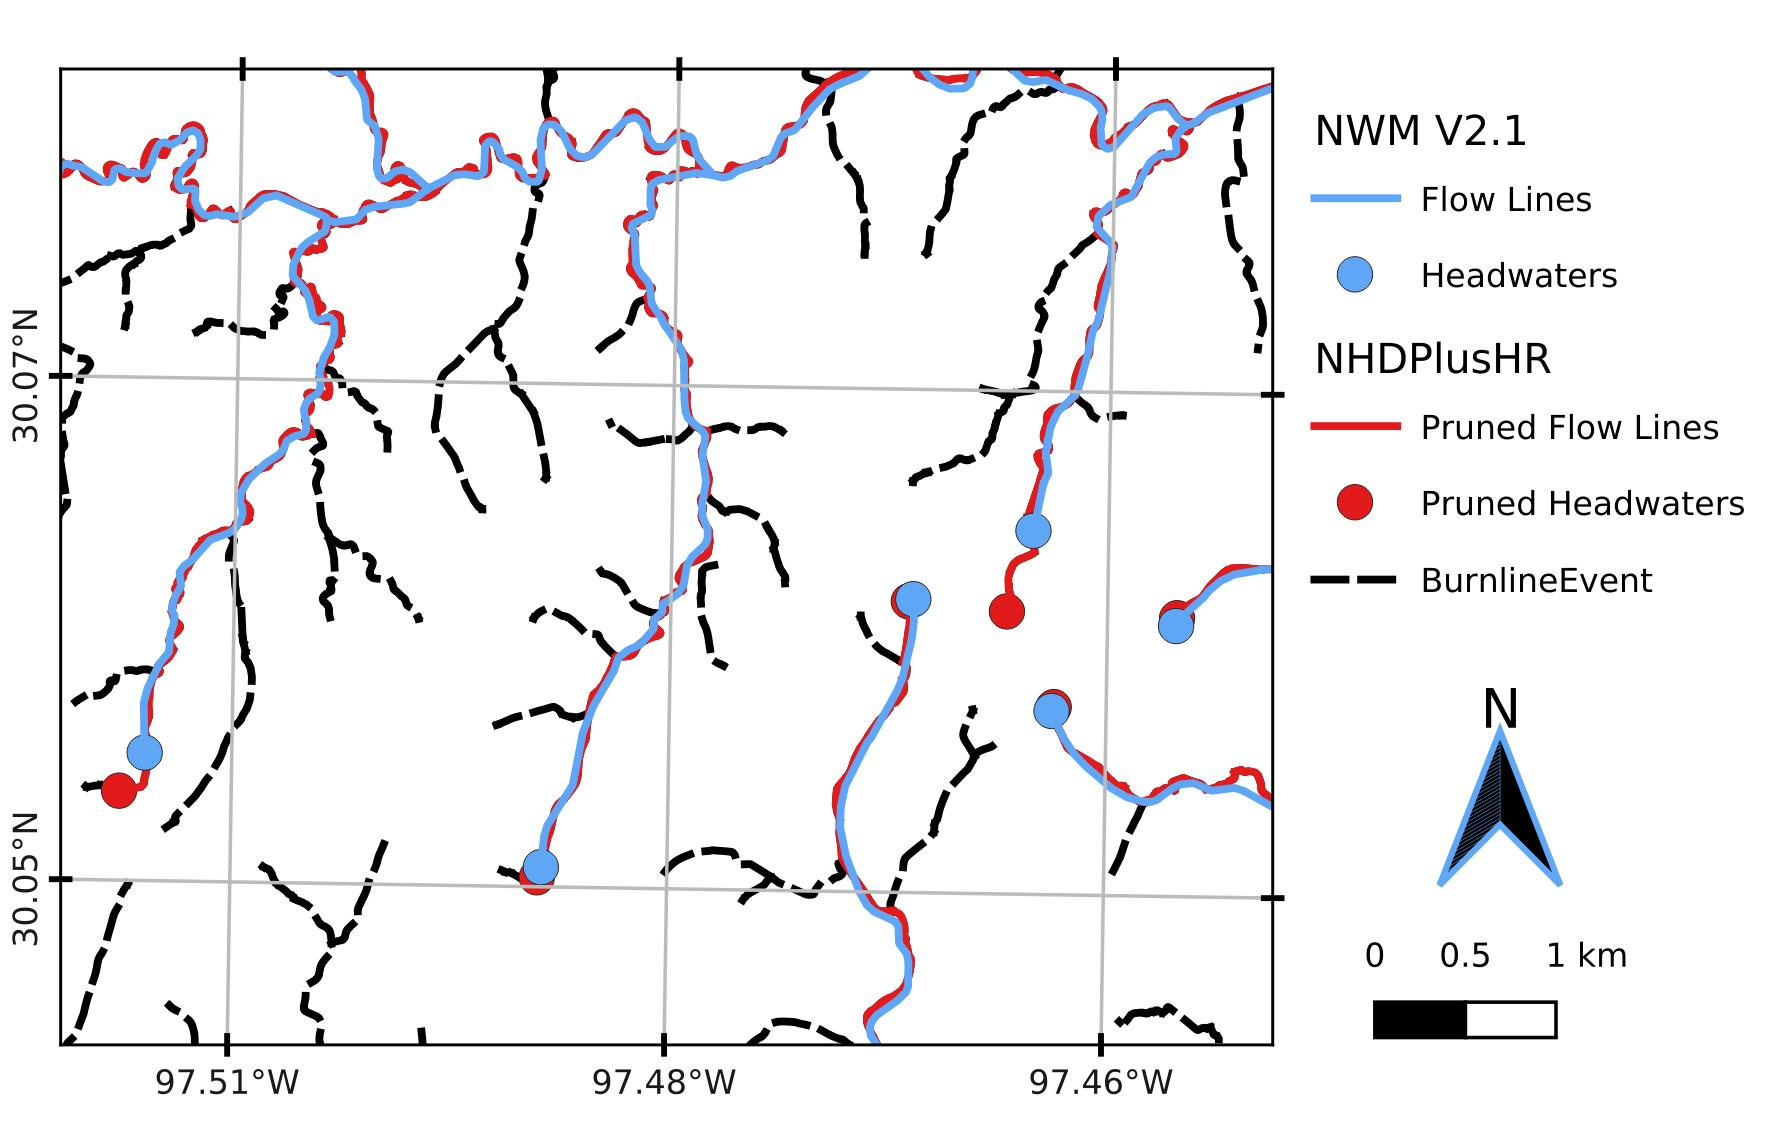
\includegraphics[scale=1.0]{figures/headwaters.jpg}
\caption{This figure illustrates some of the datasets that result from the pruning of NHDPlusHR Beta BurnlineEvents (dotted black) to the stream density of the NWM FR V2.1 density (blue).
The stream network used for forecasting, NWM FR V2.1, is of lower stream density than that of the NHDPlusHR which has better agreement with the thalweg locations in the DEM used.
Thus, we opt to trim the NHDPlusHR network to match the general location and density of the NWM network.
The nearest neighbor segment in the NHDPlusHR of each NWM headwater locations and the nearest point on that segment is determined to match the closest point to that of the NWM headwater.
These points are then traversed downstream and any segments not traversed are removed.
The resulting stream network (red) matches the drainage density of NWM V2.1 while corresponding spatially with the NHDPlusHR BurnlineEvents.}
\label{fig:stream_density_pruning}
\end{figure}
%

The reduced density stream network is then utilized to hydro-enforce the DEM with a methodology developed by \citeA{hellweger1997agree} known as the AGREE DEM Surface Reconditioning System. 
The AGREE algorithm seeks to burn artificially deep thalweg elevations by a uniform value known as sharp drop. 
The modification continues by excavating an area of a given buffer distance from the thalweg by a depth proportional to the distance from the channel given by the smooth drop and buffer distance. 
The resulting enforcement of the thalweg and general bathymetric region results in a cross-section resembling an inverted triangular notch shape with a significantly lower elevation along the thalweg line only.
In total, the AGREE algorithm requires three parameters including the buffer distance, smooth drop, and sharp drop which were set to fixed values of 70 m, 1000 m, and 10 m, respectively, but available to the user via the parameter file.
While the values for these parameters are critical to the inundation extents produced, especially for lower flow rates where bathymetric information has more influence, finding their optimal values for OWP FIM was not done since it was out of the main scientific scope of this article.
Using the AGREE method as opposed to simple thalweg burning techniques helps prevent distortions in the delineation of streams as well as the catchment boundaries \cite{saunders1995grid,saunders1996gis,mizgalewicz1996modeling,hellweger1997agree,quenzer1998gis,baker2006comparison}.
\citeA{baker2006comparison} noted AGREE produced satisfactory results when compared to other enforcement techniques especially when computational costs are considered. 
Downsides to the technique include the possibility of exhibiting parallel streams where the burned stream and real stream are both represented \cite{hellweger1997agree,saunders1999preparation} and some distortion of the catchment boundaries can also be observed \cite{saunders1999preparation,saunders1996gis}.
Some of these drawbacks are addressed by additional conditioning techniques applied in the methodology.
%%%%%%%%%%%%%%%%%%%%%%%%%%%%%%%%%%%%%%%%%%%%%%%%%%%%%%%%%%%%%%%%
\section{Flow Directions and Flats Resolution}
\label{sec:app_flow_direction_and_flat_resolution}
%%%%%%%%%%%%%%%%%%%%%%%%%%%%%%%%%%%%%%%%%%%%%%%%%%%%%%%%%%%%%%%%
%
To facilitate the generation of a connected stream network and its associated catchments from the conditioned DEM, the depression-filled DEM is used to derive connectivity in the form of D-8 flow directions.
D-8 seeks to allocate a drainage direction for every pixel based on the adjacent eight pixel neighborhood with the steepest slope \cite{o1984extraction}.
The horizontal component of slope is defined as one for the four neighboring pixels in the main cardinal directions while the intercardinal pixels are designated a horizontal component of $\sqrt{2}$ by means of the Pythagorean theorem. 
Flow directions are derived for non-depression filled regions trivially with the above procedure but to define connectivity for every grid cell the remaining flats corresponding to depression-filled cells must be resolved.

Flat resolution from flats endemic to the DEM or from depression filled regions is a costly, non-trivial procedure which was originally addressed by \citeA{garbrecht1997assignment} where flats are resolved by incrementing elevations iteratively.
Software implementations have developed means to partition the problem and resolve flats iteratively with communication across processes \cite{tarboton2009generalized,tesfa2011extraction,wallis2009parallel,tarboton2005terrain}.
The excessive iteration and communication leads to poor computational performance which motivated further work on how to optimize flat resolution \cite{survila2016scalable,barnes2014efficient}.
The established literature in this niche field of hydrology discusses how prevalent flats can be in given study areas and how difficult the problem is from both computational and hydrologic stand-points \cite{garbrecht1997assignment,tarboton2009generalized,tarboton2005terrain,survila2016scalable,barnes2014efficient,tesfa2011extraction,wallis2009parallel}.
OWP FIM utilized a CyberGIS implementation of the D-8 flow direction algorithm with the accelerated resolution of flats which we found to be very efficient and effective \cite{survila2016scalable,cybergis2016}.